\documentclass[11pt,a4paper]{article}
\usepackage[english,greek]{babel}
\usepackage[utf8]{inputenc}
\usepackage{nimbusserif}
\usepackage[T1]{fontenc}
\usepackage[left=1.50cm, right=1.50cm, top=2.00cm, bottom=2.00cm]{geometry}
\usepackage{amsmath}
\let\myBbbk\Bbbk
\let\Bbbk\relax
\usepackage[amsbb,subscriptcorrection,zswash,mtpcal,mtphrb,mtpfrak]{mtpro2}
\usepackage{graphicx,multicol,multirow,enumitem,tabularx,mathimatika,gensymb,venndiagram,hhline,longtable,tkz-euclide,fontawesome5,eurosym,tcolorbox,tabularray}
\usepackage[explicit]{titlesec}
\tcbuselibrary{skins,theorems,breakable}
\usepgfplotslibrary{fillbetween}

% Tasks Package for Horizontal MCQs
\usepackage{tasks}
\settasks{label-format=\bfseries, label-offset=1em}

\usepackage{pgfplots}
\pgfplotsset{compat=1.18}
\pgfkeys{/pgfplots/aks_on/.style={axis lines=center,
xlabel style={at={(current axis.right of origin)},xshift=1.5ex,anchor=center},
ylabel style={at={(current axis.above origin)},yshift=1.5ex, anchor=center}}}
\pgfkeys{/pgfplots/grafikh parastash/.style={red!80!black,line width=.4mm,samples=200}}

\newlist{rlist}{enumerate}{3}
\setlist[rlist]{itemsep=0mm,label=\roman*.}
\newlist{alist}{enumerate}{3}
\setlist[alist]{itemsep=0mm,label=\alph*.}
\newlist{askhseis}{enumerate}{3}
\setlist[askhseis]{label={\Large\thesection}.\arabic*.}
\renewcommand{\textstigma}{\textsigma\texttau}

\newcommand{\kerkissans}[1]{{\fontfamily{maksf}\selectfont \textbf{#1}}}
\renewcommand{\textdexiakeraia}{}

\newcommand{\dint}{\displaystyle\int}

\begin{document}

\title{\vspace{-2cm}\kerkissans{\textbf{Επαναληπτικά Θέματα Γ Λυκείου - Θεωρία (Πολλαπλής Επιλογής)}}\vspace{-0.5cm}}
\date{}
\maketitle

\noindent \kerkissans{\textbf{ΟΔΗΓΙΕΣ:}} Να επιλέξετε τη σωστή απάντηση σε καθεμία από τις παρακάτω ερωτήσεις. Σε κάθε ερώτηση υπάρχει \textbf{ακριβώς μία} σωστή επιλογή.

\vspace{0.4cm}

\begin{enumerate}[label=\textbf{\arabic*.}, itemsep=4mm]
    % ----------------- GENERAL THEORY ----------------- %
    \item Έστω οι συναρτήσεις $f, g$. Το πεδίο ορισμού της σύνθεσης $f \circ g$ ορίζεται ως:
    \begin{tasks}[label=\let\textdexiakeraia\relax\alph*.](2)
        \task $\big\{x \in D_f \mid g(x) \in D_g\big\}$
        \task $\big\{x \in D_g \mid f(x) \in D_f\big\}$
        \task $\big\{x \in D_g \mid g(x) \in D_f\big\}$
        \task $\big\{x \in D_f \mid f(x) \in D_g\big\}$
    \end{tasks}

    \item Αν $\lim\limits_{x\to x_0} f(x) = -\infty$, τότε για τιμές του $x$ "πολύ κοντά" στο $x_0$, ισχύει:
    \begin{tasks}[label=\let\textdexiakeraia\relax\alph*.](4)
        \task $f(x) > 0$
        \task $f(x) < 0$
        \task $f(x) = 0$
        \task $\lim\limits f(x) \in \mathbb{R}$
    \end{tasks}

    \item Αν $\lim\limits_{x\to x_0} f(x) = 0$ και $\lim\limits_{x\to x_0} g(x) = +\infty$, τότε το $\lim\limits_{x\to x_0} [f(x)g(x)]$ είναι:
    \begin{tasks}[label=\let\textdexiakeraia\relax\alph*.](4)
        \task Πάντα $0$
        \task Πάντα $+\infty$
        \task Πάντα $-\infty$
        \task Μορφή $0 \cdot (\pm \infty)$
    \end{tasks}

    \item Το βασικό τριγωνομετρικό όριο $\lim\limits_{x\to 0} \frac{\hm x}{x}$ ισούται με:
    \begin{tasks}[label=\let\textdexiakeraia\relax\alph*.](4)
        \task $0$
        \task $+\infty$
        \task $1$
        \task Δεν υπάρχει
    \end{tasks}

    \item Για μια συνάρτηση 1-1 ισχύει απαραίτητα ότι:
    \begin{tasks}[label=\let\textdexiakeraia\relax\alph*.](2)
        \task Είναι γνησίως μονότονη.
        \task $f(x_1) \ne f(x_2) \implies x_1 \ne x_2$.
        \task $f(x_1) = f(x_2) \implies x_1 = x_2$.
        \task Tα $C_f, C_{f^{-1}}$ τέμνονται αποκλειστικά στη διχοτόμο $y=x$.
    \end{tasks}

    \item Σύμφωνα με το θεώρημα ενδιάμεσων τιμών, η $f(x)$ παίρνει:
    \begin{tasks}[label=\let\textdexiakeraia\relax\alph*.](2)
        \task Μόνο τιμές γύρω από το μηδέν.
        \task Όλες τις τιμές μεταξύ $f(\alpha)$ και $f(\beta)$ (ως συνεχής).
        \task Μέγιστη και ελάχιστη τιμή.
        \task Μόνο θετικές τιμές.
    \end{tasks}

    \item Μία συνεχής συνάρτηση στο κλειστό $[\alpha, \beta]$:
    \begin{tasks}[label=\let\textdexiakeraia\relax\alph*.](2)
        \task Μπορεί να διαπερνά τον άξονα χωρίς ρίζα.
        \task Είναι 1-1.
        \task Παίρνει υποχρεωτικά μέγιστη (Μ) και ελάχιστη (m) τιμή.
        \task Δεν έχει τοπικά ακρότατα.
    \end{tasks}

    \item Για ποια μορφή \textbf{δεν} μπορούμε να εφαρμόσουμε άμεσα τον κανόνα του L'Hospital;
    \begin{tasks}[label=\let\textdexiakeraia\relax\alph*.](4)
        \task $\frac{0}{0}$
        \task $\frac{+\infty}{+\infty}$
        \task $\frac{-\infty}{+\infty}$
        \task $0 \cdot \infty$
    \end{tasks}

    \item Αν η συνάρτηση είναι παραγωγίσιμη σε ένα σημείο $x_0$, τότε:
    \begin{tasks}[label=\let\textdexiakeraia\relax\alph*.](2)
        \task Υποχρεωτικά $f'(x_0) = 0$.
        \task Είναι οπωσδήποτε συνεχής στο $x_0$.
        \task Μπορεί να έχει πλευρικά όρια που διαφέρουν.
        \task Παρουσιάζει ακρότατο.
    \end{tasks}

    \item Ο γεωμετρικός ορισμός της $f'(x_0)$ ταυτίζεται με:
    \begin{tasks}[label=\let\textdexiakeraia\relax\alph*.](2)
        \task Τον άξονα συμμετρίας της συνάρτησης.
        \task Το εμβαδόν υπό την καμπύλη.
        \task Το συντελεστή διεύθυνσης $\lambda$ της εφαπτομένης της $C_f$ στο $x_0$.
        \task Την ελάχιστη τιμή της $f$.
    \end{tasks}

    \item Αν $x_0$ είναι εσωτερικό σημείο και τοπικό ακρότατο της $f$, και η $f$ παραγωγίζεται στο $x_0$, τότε:
    \begin{tasks}[label=\let\textdexiakeraia\relax\alph*.](4)
        \task $f'(x_0) > 0$
        \task $f'(x_0) < 0$
        \task $f'(x_0) = 0$
        \task Δεν εξάγεται συμπέρασμα
    \end{tasks}

    \item Ποια συνθήκη ΔΕΝ ανήκει στο Θεώρημα του Rolle για το διάστημα $[\alpha, \beta]$;
    \begin{tasks}[label=\let\textdexiakeraia\relax\alph*.](2)
        \task H $f$ είναι συνεχής στο $[\alpha, \beta]$.
        \task H $f$ είναι παραγωγίσιμη στο $[\alpha, \beta]$.
        \task $f(\alpha) = f(\beta)$.
        \task H $f$ είναι παραγωγίσιμη στο $(\alpha, \beta)$.
    \end{tasks}

    \item Αν $f'(x) = 0$ για ΚΑΘΕ $x$ σε ένα \textbf{διάστημα} $\Delta$, τότε:
    \begin{tasks}[label=\let\textdexiakeraia\relax\alph*.](2)
        \task H $f$ είναι γνησίως αύξουσα στο $\Delta$.
        \task H $f$ είναι σταθερή συνάρτηση στο $\Delta$.
        \task H $f$ ταλαντώνεται στο $\Delta$.
        \task H $f$ είναι εξίσωση ευθείας με $a \ne 0$.
    \end{tasks}

    \item Αν $f''(x) > 0$ για κάθε $x \in \Delta$, η γραφική παράσταση της $f$ αναφορικά με την εφαπτομένη της:
    \begin{tasks}[label=\let\textdexiakeraia\relax\alph*.](2)
        \task Βρίσκεται χαμηλότερα, με εξαίρεση το σημείο επαφής.
        \task Βρίσκεται ψηλότερα, με εξαίρεση το σημείο επαφής.
        \task Διαπερνάται από αυτή σε κάθε σημείο.
        \task Συμπίπτει με αυτή.
    \end{tasks}

    \item Το σημείο $M(x_0, f(x_0))$ λέγεται σημείο καμπής αν:
    \begin{tasks}[label=\let\textdexiakeraia\relax\alph*.](2)
        \task H $f$ παρουσιάζει τοπικό μέγιστο και τοπικό ελάχιστο.
        \task H $C_f$ έχει εφαπτομένη και αλλάζει κυρτότητα εκατέρωθεν του $x_0$.
        \task $f'(x_0) = 0$ αυστηρά.
        \task $f(x_0) = 0$.
    \end{tasks}

    \item Η ιδιότητα $\dint_\alpha^\beta f(x) dx = - \dint_\beta^\alpha f(x) dx$ ισχύει:
    \begin{tasks}[label=\let\textdexiakeraia\relax\alph*.](2)
        \task Μόνο αν $\alpha > \beta$.
        \task Μόνο αν $f(x) \ge 0$.
        \task Εφόσον η $f$ είναι συνεχής, για οποιαδήποτε $\alpha, \beta$.
        \task Ποτέ.
    \end{tasks}

    \item Το $\dint_\alpha^\beta c dx$ (όπου $c$ σταθερός πραγματικός αριθμός), ισούται με:
    \begin{tasks}[label=\let\textdexiakeraia\relax\alph*.](4)
        \task $c$
        \task $c\cdot x$
        \task $c(\beta - \alpha)$
        \task $\beta - \alpha$
    \end{tasks}

    \item Η παράγωγος της ολοκληρωτικής συνάρτησης $F(x) = \dint_\alpha^x f(t) dt$ (με $f$ συνεχή) είναι:
    \begin{tasks}[label=\let\textdexiakeraia\relax\alph*.](4)
        \task $F'(x) = 0$
        \task $F'(x) = f(t)$
        \task $F'(x) = f(x)$
        \task $F'(x) = f(x) - f(\alpha)$
    \end{tasks}

    \item Ο τύπος ολοκλήρωσης κατά παράγοντες είναι:
    \begin{tasks}[label=\let\textdexiakeraia\relax\alph*.](2)
        \task $\dint_\alpha^\beta f(x)g'(x) dx = f(\beta)g(\beta) - \dint_\alpha^\beta f'(x)g(x) dx$
        \task $\dint_\alpha^\beta f(x)g'(x) dx = [f(x)g(x)]_\alpha^\beta - \dint_\alpha^\beta f'(x)g(x) dx$
        \task $\dint_\alpha^\beta f'(x)g'(x) dx = f(x)g(x)$
        \task $\dint_\alpha^\beta (f(x)g(x))' dx = f(x) g(x)$
    \end{tasks}

    \item Έστω $f(x) \ge 0$. Το εμβαδόν του χωρίου μεταξύ $C_f$, άξονα $x'x$ και ευθειών $x=\alpha, x=\beta$ (με $\alpha<\beta$) δίνεται από:
    \begin{tasks}[label=\let\textdexiakeraia\relax\alph*.](4)
        \task $E = \dint_\beta^\alpha f(x) dx$
        \task $E = - \dint_\alpha^\beta f(x) dx$
        \task $E = \dint_\alpha^\beta f(x) dx$
        \task $E = |f(\alpha) - f(\beta)|$
    \end{tasks}

    \item Αν $\dint_\alpha^\beta f(x) dx = 0$ και η $f$ είναι συνεχής με $f(x) \ge 0$, τότε αναγκαστικά:
    \begin{tasks}[label=\let\textdexiakeraia\relax\alph*.](2)
        \task $f(x) = 0$ για κάθε $x \in [\alpha, \beta]$.
        \task H $f$ είναι σταθερή αλλά όχι μηδενική.
        \task $\alpha = 0$ ή $\beta = 0$.
        \task H $f$ είναι περιττή.
    \end{tasks}

    \item Το ολοκλήρωμα $\dint_{a}^{\beta} f(\hm(x)) \syn(x) dx$ αντιμετωπίζεται καλώντας:
    \begin{tasks}[label=\let\textdexiakeraia\relax\alph*.](2)
        \task Παραγοντική ολοκλήρωση.
        \task Αντικατάσταση $u = \hm x$.
        \task Αντικατάσταση $u = \syn x$.
        \task Αδύνατον.
    \end{tasks}

    \item Μια ασύμπτωτη ευθεία πλάγιας μορφής ορίζεται από τη σχέση $\lim\limits [\dots] = 0$. Το μέσα όριο είναι:
    \begin{tasks}[label=\let\textdexiakeraia\relax\alph*.](4)
        \task $f(x) \cdot (\lambda x + \mu)$
        \task $f(x) - \lambda x$
        \task $f(x) - \lambda$
        \task $f(x) - (\lambda x + \mu)$
    \end{tasks}

    \item Η κατακόρυφη ασύμπτωτη εμφανίζεται συχνότερα στα σημεία $x_0$ όπου:
    \begin{tasks}[label=\let\textdexiakeraia\relax\alph*.](2)
        \task Ο αριθμητής μηδενίζεται και ο παρονομαστής όχι.
        \task Η συνάρτηση παρουσιάζει ελάχιστο.
        \task Το πλευρικό όριο καταλήγει σε $+\infty$ ή $-\infty$.
        \task Ορίζεται η συνάρτηση χωρίς ανωμαλίες.
    \end{tasks}

    \item Η εφαπτομένη της γραφικής παράστασης $C_f$ στο $A(x_0, f(x_0))$ τέμνει τον άξονα $x'x$ υπό γωνία $\omega$. Ισχύει πάντοτε:
    \begin{tasks}[label=\let\textdexiakeraia\relax\alph*.](4)
        \task $f'(x_0) = \hm \omega$
        \task $f'(x_0) = \ef \omega$
        \task $f'(x_0) = \omega$
        \task $f'(x_0) = \syn \omega$
    \end{tasks}


    % ----------------- GRAPHICAL (5 Questions) ----------------- %
    \newpage
    \item Παρατηρήστε την παρακάτω γραφική παράσταση της \textbf{παραγώγου} $f'(x)$ μιας συνεχούς συνάρτησης $f$.
    \begin{center}
    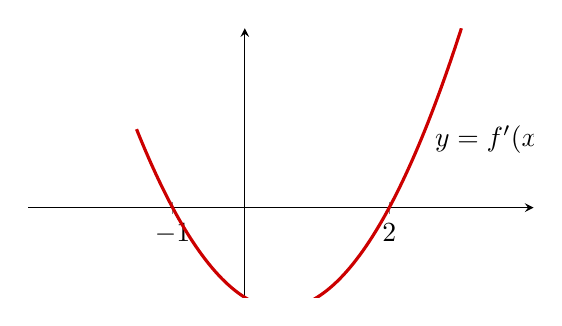
\begin{tikzpicture}
      \begin{axis}[
          aks_on,
          xmin=-3, xmax=4,
          ymin=-2, ymax=4,
          xtick={-1, 2}, xticklabels={$-1$, $2$},
          ytick=\empty,
          width=8cm, height=5cm
      ]
      \addplot[grafikh parastash, domain=-1.5:3, samples=100] {(x+1)*(x-2)};
      \node[anchor=south west] at (axis cs:2.5, 1) {$y = f'(x)$};
      \end{axis}
    \end{tikzpicture}
    \end{center}
    Σε ποιο από τα παρακάτω διαστήματα η αρχική συνάρτηση $f(x)$ είναι γνησίως φθίνουσα;
    \begin{tasks}[label=\let\textdexiakeraia\relax\alph*.](4)
        \task $[ -1, 2 ]$
        \task $(-\infty, -1]$
        \task $[2, +\infty)$
        \task $\mathbb{R}$
    \end{tasks}

    \item Στο παρακάτω σχήμα απεικονίζεται η \textbf{δεύτερη παράγωγος} $f''(x)$. 
    \begin{center}
    \begin{tikzpicture}
      \begin{axis}[
          aks_on,
          xmin=-2, xmax=4,
          ymin=-2, ymax=3,
          xtick={1}, xticklabels={$1$},
          ytick=\empty,
          width=8cm, height=5cm
      ]
      \addplot[grafikh parastash, domain=-1:3, samples=2] {x-1};
      \node[anchor=north west] at (axis cs:1.5, 2) {$y = f''(x)$};
      \end{axis}
    \end{tikzpicture}
    \end{center}
    Ποιος ισχυρισμός για την αρχική συνάρτηση $f(x)$ είναι απόλυτα ακριβής (δεχόμενοι ότι ορίζεται η εφαπτομένη της στο 1);
    \begin{tasks}[label=\let\textdexiakeraia\relax\alph*.](2)
        \task Η $f$ παρουσιάζει τοπικό ελάχιστο στο $x_0 = 1$.
        \task Το σημείο με τετμημένη $x_0 = 1$ είναι θέση σημείου καμπής της $f$.
        \task Η $f$ είναι κοίλη (στρέφει τα κοίλα κάτω) στο $[1, +\infty)$.
        \task Η πρώτη παράγωγος είναι αδύνατον να βρεθεί.
    \end{tasks}

    \item Δίνεται η γραφική παράσταση της συνάρτησης $f(x)$ με μία οριζόντια ασύμπτωτη:
    \begin{center}
    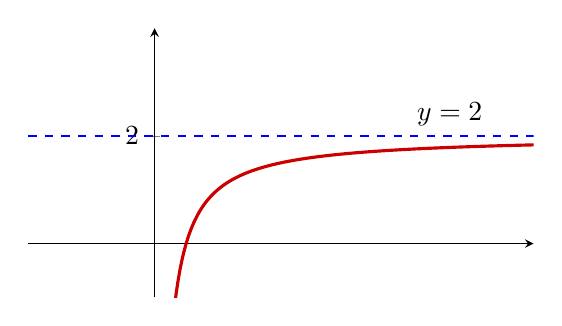
\begin{tikzpicture}
      \begin{axis}[
          aks_on,
          xmin=-2, xmax=6,
          ymin=-1, ymax=4,
          xtick=\empty, ytick={2}, yticklabels={$2$},
          width=8cm, height=5cm
      ]
      \addplot[grafikh parastash, domain=0.2:6] {2 - 1/x};
      \draw[dashed, line width=0.3mm, blue] (axis cs:-2, 2) -- (axis cs:6, 2);
      \node[anchor=south west] at (axis cs:4, 2) {$y = 2$};
      \end{axis}
    \end{tikzpicture}
    \end{center}
    Από την ερμηνεία του γραφήματος, ποιο είναι το όριο $\lim\limits_{x\to +\infty} f(x)$;
    \begin{tasks}[label=\let\textdexiakeraia\relax\alph*.](4)
        \task $-\infty$
        \task $0$
        \task $2$
        \task $+\infty$
    \end{tasks}

    \item Απεικονίζεται η \textbf{πρώτη παράγωγος} $f'(x)$, η οποία είναι γραμμική γνησίως φθίνουσα, τέμνοντας τον άξονα στο $x=3$.
    \begin{center}
    \begin{tikzpicture}
      \begin{axis}[
          aks_on,
          xmin=-1, xmax=5,
          ymin=-3, ymax=3,
          xtick={3}, xticklabels={$3$},
          ytick=\empty,
          width=8cm, height=5cm
      ]
      \addplot[grafikh parastash, domain=0:5] {-x+3};
      \node[anchor=south west] at (axis cs:1, 2.5) {$y = f'(x)$};
      \end{axis}
    \end{tikzpicture}
    \end{center}
    Τι συμπεραίνουμε για το ακρότατο της $f$ στη θέση $x=3$;
    \begin{tasks}[label=\let\textdexiakeraia\relax\alph*.](2)
        \task H $f$ παρουσιάζει τοπικό ελάχιστο διότι το γράφημα της $f'$ κατεβαίνει.
        \task H $f$ παρουσιάζει τοπικό μέγιστο διότι η $f'$ αλλάζει πρόσημο από $+$ σε $-$.
        \task Είναι σημείο καμπής.
        \task Δεν είναι ακρότατο αφού η εφαπτομένη της $f'$ δεν είναι μηδέν.
    \end{tasks}

    \item Δίνεται το εμβαδόν ενός κλειστού χωρίου $\Omega$ ανάμεσα στην καμπύλη της $f$, τον $x'x$ και τις ευθείες $x=0, x=4$.
    \begin{center}
    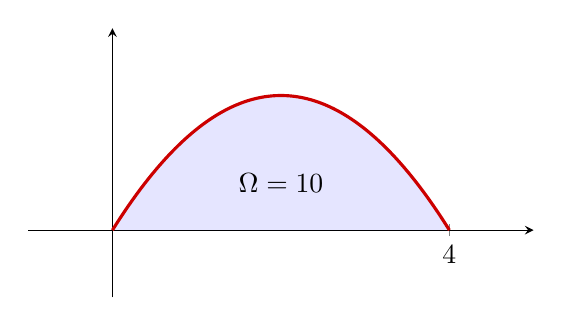
\begin{tikzpicture}
      \begin{axis}[
          aks_on,
          xmin=-1, xmax=5,
          ymin=-1, ymax=3,
          xtick={0, 4}, xticklabels={$0$, $4$},
          ytick=\empty,
          width=8cm, height=5cm
      ]
      \addplot[name path=f, grafikh parastash, domain=0:4] {0.5*x*(4-x)};
      \path[name path=axis] (axis cs:0,0) -- (axis cs:4,0);
      \addplot[blue, opacity=0.1] fill between[of=f and axis];
      \node at (axis cs:2, 0.7) {$\Omega = 10$};
      \end{axis}
    \end{tikzpicture}
    \end{center}
    Βασιζόμενοι στο σχήμα (όπου $f(x)>0$ στο $(0,4)$), αν $F$ μια αρχική της $f$, ισχύει:
    \begin{tasks}[label=\let\textdexiakeraia\relax\alph*.](2)
        \task $F(4) - F(0) = -10$
        \task $F'(4) - F'(0) = 10$
        \task $\dint_0^4 f(x) dx = 10 \implies F(4) - F(0) = 10$
        \task $\dint_4^0 f(x) dx = 10$
    \end{tasks}


    % ==================== ΝΕΕΣ ΕΡΩΤΗΣΕΙΣ 31-50 ==================== %

    \item Αν $f'(x_0) = 0$ και $f''(x_0) > 0$, τότε στο $x_0$ η $f$:
    \begin{tasks}[label=\let\textdexiakeraia\relax\alph*.](2)
        \task Παρουσιάζει τοπικό μέγιστο.
        \task Παρουσιάζει τοπικό ελάχιστο.
        \task Παρουσιάζει σημείο καμπής.
        \task Δεν εξάγεται συμπέρασμα.
    \end{tasks}

    \item Η εξίσωση της εφαπτομένης της $C_f$ στο σημείο $(x_0, f(x_0))$ δίνεται από τη σχέση:
    \begin{tasks}[label=\let\textdexiakeraia\relax\alph*.](2)
        \task $y = f(x_0) + f'(x)(x - x_0)$
        \task $y - f(x_0) = f'(x_0)(x - x_0)$
        \task $y = f'(x_0) \cdot x + f(x_0)$
        \task $y = f(x_0)(x - x_0)$
    \end{tasks}

    \item Αν $F_1, F_2$ δύο παράγουσες (αρχικές) της ίδιας συνάρτησης $f$ σε ένα διάστημα $\Delta$, τότε:
    \begin{tasks}[label=\let\textdexiakeraia\relax\alph*.](2)
        \task $F_1(x) = F_2(x)$ για κάθε $x \in \Delta$.
        \task $F_1(x) - F_2(x) = c$ (σταθερά) για κάθε $x \in \Delta$.
        \task $F_1'(x) \ne F_2'(x)$ σε κάποιο $x$.
        \task $F_1 \cdot F_2 = c$ (σταθερά).
    \end{tasks}

    \item Αν $f$ συνεχής στο $[\alpha, \beta]$ και $m \le f(x) \le M$ για κάθε $x \in [\alpha, \beta]$, τότε:
    \begin{tasks}[label=\let\textdexiakeraia\relax\alph*.](2)
        \task $\dint_\alpha^\beta f(x) dx = m(\beta - \alpha)$
        \task $m(\beta-\alpha) \le \dint_\alpha^\beta f(x) dx \le M(\beta-\alpha)$
        \task $\dint_\alpha^\beta f(x)dx \ge M(\beta-\alpha)$
        \task Δεν μπορεί να εκτιμηθεί το ολοκλήρωμα.
    \end{tasks}

    \item Η παράγωγος της σύνθετης συνάρτησης $f(g(x))$ ισούται με:
    \begin{tasks}[label=\let\textdexiakeraia\relax\alph*.](2)
        \task $f'(x) \cdot g'(x)$
        \task $f'(g(x)) \cdot g'(x)$
        \task $f(g'(x))$
        \task $f'(g(x)) + g'(x)$
    \end{tasks}

    \item To $\displaystyle\lim_{x\to 0} \frac{e^x - 1}{x}$ ισούται με:
    \begin{tasks}[label=\let\textdexiakeraia\relax\alph*.](4)
        \task $0$
        \task $1$
        \task $e$
        \task $+\infty$
    \end{tasks}

    \item Ποια είναι η παράγωγος της $f(x) = \ln|g(x)|$, αν $g(x) \ne 0$ και $g$ παραγωγίσιμη;
    \begin{tasks}[label=\let\textdexiakeraia\relax\alph*.](4)
        \task $\frac{1}{g(x)}$
        \task $\frac{g'(x)}{g(x)}$
        \task $\frac{1}{|g(x)|}$
        \task $g'(x) \cdot \ln|g(x)|$
    \end{tasks}

    \item Αν η $f$ είναι συνεχής στο $[\alpha, \beta]$ και $\dint_\alpha^\beta f(x)dx > 0$ (με $\alpha < \beta$), τότε:
    \begin{tasks}[label=\let\textdexiakeraia\relax\alph*.](2)
        \task $f(x) > 0$ σε κάθε $x \in [\alpha, \beta]$.
        \task Υπάρχει $x_0 \in [\alpha, \beta]$ με $f(x_0) > 0$.
        \task $f(\alpha) > 0$ και $f(\beta) > 0$.
        \task H $f$ δεν έχει ρίζες.
    \end{tasks}

    \item Αν $\lim\limits_{x\to x_0} f(x) = \ell$ και $\lim\limits_{x\to x_0} g(x) = m$ πεπερασμένα, ποια ιδιότητα ΔΕΝ ισχύει γενικά;
    \begin{tasks}[label=\let\textdexiakeraia\relax\alph*.](2)
        \task $\lim (f+g) = \ell + m$
        \task $\lim (f \cdot g) = \ell \cdot m$
        \task $\lim (f/g) = \ell/m$
        \task $\lim (f - g) = \ell - m$
    \end{tasks}

    \item Αν $f$ άρτια και ολοκληρώσιμη στο $[-\alpha, \alpha]$ ($\alpha > 0$), τότε:
    \begin{tasks}[label=\let\textdexiakeraia\relax\alph*.](2)
        \task $\dint_{-\alpha}^{\alpha} f(x) dx = 0$
        \task $\dint_{-\alpha}^{\alpha} f(x) dx = 2\dint_0^{\alpha} f(x) dx$
        \task $\dint_{-\alpha}^{\alpha} f(x) dx = \alpha \cdot f(0)$
        \task H $f$ δεν είναι ολοκληρώσιμη.
    \end{tasks}

    \item Κατά την ολοκλήρωση με αντικατάσταση $u = g(x)$, αλλάζουν:
    \begin{tasks}[label=\let\textdexiakeraia\relax\alph*.](2)
        \task Μόνο η μεταβλητή ολοκλήρωσης.
        \task H μεταβλητή ολοκλήρωσης και τα όρια ολοκλήρωσης.
        \task Μόνο τα όρια ολοκλήρωσης.
        \task Τίποτα.
    \end{tasks}

    \item Αν $f$ συνεχής στο $[a,b]$ με $f(a) \cdot f(b) < 0$, τότε:
    \begin{tasks}[label=\let\textdexiakeraia\relax\alph*.](2)
        \task Η $f$ είναι μονότονη.
        \task Η εξίσωση $f(x) = 0$ έχει τουλάχιστον μια ρίζα στο $(a,b)$.
        \task Η $f$ μηδενίζεται ακριβώς μία φορά.
        \task Η $f$ δεν είναι παραγωγίσιμη στο $(a,b)$.
    \end{tasks}

    \item Αν $\lim\limits_{x\to +\infty} \frac{f(x)}{x} = \lambda$ και $\lim\limits_{x\to +\infty} (f(x) - \lambda x) = \mu$, η $C_f$ έχει:
    \begin{tasks}[label=\let\textdexiakeraia\relax\alph*.](2)
        \task Κατακόρυφη ασύμπτωτη $x = \lambda$.
        \task Οριζόντια ασύμπτωτη $y = \mu$.
        \task Πλάγια ασύμπτωτη $y = \lambda x + \mu$ στο $+\infty$.
        \task Καμία ασύμπτωτη.
    \end{tasks}

    \item Αν η παράγωγος $f'(x_0)$ ΔΕΝ υπάρχει (ενώ η $f$ είναι συνεχής στο $x_0$), τότε στο $x_0$:
    \begin{tasks}[label=\let\textdexiakeraia\relax\alph*.](2)
        \task Η $f$ δεν μπορεί να έχει ακρότατο.
        \task Η $f$ μπορεί να έχει ακρότατο (π.χ. $f(x)=|x|$ στο $0$).
        \task Η $f$ είναι αναγκαστικά σταθερή κοντά στο $x_0$.
        \task Η $f$ δεν ορίζεται στο $x_0$.
    \end{tasks}

    \item Ποια σχέση είναι σωστή μεταξύ θεωρημάτων;
    \begin{tasks}[label=\let\textdexiakeraia\relax\alph*.](2)
        \task Το Θ.Μ.Τ. είναι ειδική περίπτωση του Rolle, δηλαδή Θ.Μ.Τ. $\subset$ Rolle.
        \task Το Rolle είναι ειδική περίπτωση του Θ.Μ.Τ., δηλαδή Rolle $\subset$ Θ.Μ.Τ.
        \task Τα δύο θεωρήματα είναι ανεξάρτητα.
        \task Μόνο το Rolle χρειάζεται παραγωγισιμότητα.
    \end{tasks}

    \item Αν $f$ γνησίως αύξουσα και συνεχής στο $[\alpha, \beta]$, τότε το σύνολο τιμών της $f$ είναι:
    \begin{tasks}[label=\let\textdexiakeraia\relax\alph*.](4)
        \task $(f(\alpha), f(\beta))$
        \task $[f(\alpha), f(\beta)]$
        \task $\{f(\alpha), f(\beta)\}$
        \task $\mathbb{R}$
    \end{tasks}

    \item Τo ολοκλήρωμα $\dint_1^e \frac{1}{x} dx$ ισούται με:
    \begin{tasks}[label=\let\textdexiakeraia\relax\alph*.](4)
        \task $e-1$
        \task $1$
        \task $\frac{1}{e}$
        \task $e$
    \end{tasks}

    \item Αν $f$ περιττή και ολοκληρώσιμη στο $[-\alpha, \alpha]$ ($\alpha > 0$), τότε $\dint_{-\alpha}^{\alpha} f(x) dx$ ισούται με:
    \begin{tasks}[label=\let\textdexiakeraia\relax\alph*.](4)
        \task $2 \dint_0^\alpha f(x)dx$
        \task $0$
        \task $f(\alpha) - f(-\alpha)$
        \task $\alpha$
    \end{tasks}

    \item Έστω $f$ παραγωγίσιμη με $f'(x) > 0$ για κάθε $x$ σε ένα διάστημα $\Delta$. Ποιο από τα παρακάτω ΔΕΝ ισχύει;
    \begin{tasks}[label=\let\textdexiakeraia\relax\alph*.](2)
        \task Η $f$ είναι γνησίως αύξουσα στο $\Delta$.
        \task Η $f$ αντιστρέφεται στο $\Delta$.
        \task Η $f$ είναι κυρτή στο $\Delta$.
        \task Η $f$ δεν παρουσιάζει ακρότατο στο εσωτερικό του $\Delta$.
    \end{tasks}

    \item Αν $\dint_\alpha^\beta f(x) dx = \dint_\alpha^\gamma f(x) dx + \dint_\gamma^\beta f(x) dx$ (προσθετικότητα ως προς τα όρια), αυτό ισχύει:
    \begin{tasks}[label=\let\textdexiakeraia\relax\alph*.](2)
        \task Μόνο αν $\alpha < \gamma < \beta$.
        \task Μόνο αν $f(x) \ge 0$.
        \task Για κάθε $\gamma$ πραγματικό, αρκεί η $f$ να ολοκληρώνεται.
        \task Μόνο αν η $f$ είναι μονότονη.
    \end{tasks}

\end{enumerate}

\newpage
\noindent \kerkissans{\Large{\textbf{ΑΠΑΝΤΗΤΙΚΟ ΦΥΛΛΟ}}}

\vspace{0.3cm}
\begin{tcolorbox}[colback=black!5!white, colframe=black, title=\textbf{Σωστά Γράμματα (Κλειδί)}]
\begin{multicols}{3}
\begin{itemize}[label=$-$]
    \item \textbf{1.} $\gamma$
    \item \textbf{2.} $\beta$
    \item \textbf{3.} $\delta$
    \item \textbf{4.} $\gamma$
    \item \textbf{5.} $\gamma$
    \item \textbf{6.} $\beta$
    \item \textbf{7.} $\gamma$
    \item \textbf{8.} $\delta$
    \item \textbf{9.} $\beta$
    \item \textbf{10.} $\gamma$
    \item \textbf{11.} $\gamma$
    \item \textbf{12.} $\beta$ 
    \item \textbf{13.} $\beta$
    \item \textbf{14.} $\beta$
    \item \textbf{15.} $\beta$
    \item \textbf{16.} $\gamma$
    \item \textbf{17.} $\gamma$
    \item \textbf{18.} $\gamma$
    \item \textbf{19.} $\beta$
    \item \textbf{20.} $\gamma$
    \item \textbf{21.} $\alpha$
    \item \textbf{22.} $\beta$
    \item \textbf{23.} $\delta$
    \item \textbf{24.} $\gamma$
    \item \textbf{25.} $\beta$
    \item \textbf{26.} $\alpha$ (Η $f'<0$ ανάμεσα ρίζες)
    \item \textbf{27.} $\beta$ ($f''$ τέμνει άξονα)
    \item \textbf{28.} $\gamma$
    \item \textbf{29.} $\beta$ (Η $f'$ αλλάζει από + σε -)
    \item \textbf{30.} $\gamma$ (Το ολοκλήρωμα ισούται ακριβώς 10)
    \item \textbf{31.} $\beta$ (Τοπικό ελάχιστο, κριτήριο $f''$)
    \item \textbf{32.} $\beta$ (Τύπος εφαπτομένης)
    \item \textbf{33.} $\beta$ (Δύο παράγουσες διαφέρουν κατά σταθερά)
    \item \textbf{34.} $\beta$ (Φράξη ολοκληρώματος)
    \item \textbf{35.} $\beta$ (Κανόνας αλυσίδας)
    \item \textbf{36.} $\beta$ (Βασικό εκθετικό όριο)
    \item \textbf{37.} $\beta$ (Παράγωγος σύνθετου λογαρίθμου)
    \item \textbf{38.} $\beta$ (Υπάρχει $x_0$ με $f(x_0)>0$)
    \item \textbf{39.} $\gamma$ (Αν $m=0$ δεν ισχύει)
    \item \textbf{40.} $\beta$ (Ιδιότητα άρτιας)
    \item \textbf{41.} $\beta$ (Αλλάζουν μεταβλητή και όρια)
    \item \textbf{42.} $\beta$ (Bolzano)
    \item \textbf{43.} $\gamma$ (Πλάγια ασύμπτωτη)
    \item \textbf{44.} $\beta$ (Ακρότατο χωρίς παράγωγο)
    \item \textbf{45.} $\beta$ (Rolle $\subset$ Θ.Μ.Τ.)
    \item \textbf{46.} $\beta$ (Κλειστό διάστημα, Θ.Ε.Τ.)
    \item \textbf{47.} $\beta$ ($\ln e - \ln 1 = 1$)
    \item \textbf{48.} $\beta$ (Ιδιότητα περιττής)
    \item \textbf{49.} $\gamma$ ($f'>0$ δεν συνεπάγεται κυρτότητα)
    \item \textbf{50.} $\gamma$ (Ισχύει για κάθε $\gamma$)
\end{itemize}
\end{multicols}
\end{tcolorbox}


\end{document}
